\item In \figref{fig:Fig-4.png}, the angle of elevation of the top of a tower from a point $C$ on the ground, which is $30m$ away from the foot of the tower, is $30\degree$. Find the height of the tower.      
\begin{figure}[H]
\centering
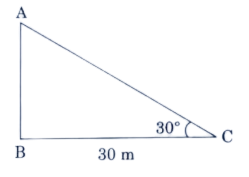
\includegraphics[width=0.75\columnwidth]{cbse-math/figs/Fig-4.png}
\caption{}      
\label{fig:Fig-4.png}
\end{figure}
\hfill\brak{10, 2020}\item A statue $1.6m$ tall, stands on the top of a pedestal. From a point on the ground, the angle of elevation of the top of the statue is $60\degree$ and from the same point the angle of elevation of the top of the pedestal is $45\degree$. Find the height of the pedestal.(Use $\sqrt{3}=1.73$)
\hfill\brak{10, 2020}
